% [R16-B] Preserve original comparison layers; administrative provenance stays in archived sources.
\section{Appendix B. Annotation-Quality Evidence}
\phantomsection
\label{app:b}
\label{sec:quality-provenance-r12}
We describe reference construction, assisted review, and the separate blinded study (Table~\ref{tab:quality-main}).

\subsection{Human Annotation and Review Coverage}
\label{sec:human-review-coverage}
The 150-sentence human reference, initial 100-sentence silver review, and separate 100-sentence post-generation review cover 350 unique sentences. The early 15-sentence assisted-review subset is included in the post-generation cohort. The additional review contributes 150 sentences: 60 cloud, 45 public-sector, and 45 listed-company sentences. Identifier and normalized-text checks excluded the original 350 sentences from this additional sample, yielding 500 sentences with human annotation or review before the blinded study. The 50-sentence blinded study has no normalized-text overlap with these cohorts, bringing coverage to 550 distinct sentences. Each sentence is counted once across annotation layers. Model-evaluation labels come from the 150-sentence human reference; the remaining cohorts serve annotation-quality assessment.

\subsection{Reference Construction and Initial Agreement}
The human reference combines 50 calibration sentences sampled from the 980-record model-disagreement queue and a separate 100-sentence challenge sample. The calibration sentences were annotated separately and adjudicated; the challenge sample was collaboratively annotated and reviewed. The authors recall machine suggestions being available during calibration, whereas an earlier protocol specifies raw-text-only coding. The available records do not resolve this discrepancy, so this stage is not treated as a blinded agreement study. All 50 calibration sentence IDs are absent from the silver training and development sets.

The finalized reference contains 415 challenge-sample spans (290 S, 83 K, 41 T, one L) and 248 calibration-sample spans (158 S, 42 K, 47 T, one L). Seven challenge sentences and one calibration sentence have no annotated span. The 150 reference sentences correspond to 61 source-document prefixes in the original corpus. These reference labels are used for model evaluation and remain separate from the individual coding and assisted-review layers.

The two available calibration annotation layers contain 211 and 230 spans, with 98 exact typed matches and F1 of 0.444. Character-level $\kappa$ is 0.567 across all 2,571 source code points, including spaces and punctuation. These retrospective estimates use available exports whose correspondence to the original frozen files has not been verified. They describe initial agreement, rather than an independent assessment of the adjudicated reference. Comparisons with that reference involve the same annotators and reflect adjudication changes; the detailed scores and supporting records are provided in the \href{https://github.com/AlfredJamesLi/chinese-skillspan-benchmark/blob/main/reproduction/annotation_documentation_20261007/README.md}{annotation documentation}.

% [R37-MOVE] Counting convention formerly repeated in the corpus chapter.
Character-level Cohen's $\kappa$ adjusts observed agreement for agreement expected by chance from the two coders' marginal label frequencies across the source character positions:
\begin{equation}
\kappa=\frac{p_o-p_e}{1-p_e},
\qquad p_e=\sum_{c\in\mathcal{C}}p_A(c)\,p_B(c).
\label{eq:character-kappa}
\end{equation}
Here, $p_o$ is the fraction of source character positions with identical labels, and $p_A(c)$ and $p_B(c)$ are the two coders' label proportions. The label set $\mathcal{C}$ comprises L/K/S/T and O. For the four-label scheme plus O, the available exports yield $p_o=0.771$ and $p_e=0.471$, giving $\kappa=0.567$. These coefficients use character positions rather than the spans counted in Eq.~\eqref{eq:micro-prf}. The 2,571 positions are nested within the 50 sampled sentences.

When both annotations of a sentence are empty, the pair contributes no span true positives. Span matching and character-level agreement use different units; optional category projections are described in the reproduction materials.

\subsection{Post-Generation Assisted Review}
The 100-sentence post-generation review sample was stratified by source, empty/nonempty annotation, and text length. The sampling frame contained 2,179 eligible records after excluding 100 initially reviewed records, 100 reserved for an earlier pilot, and 72 pending records from the 2,451-record original silver pool. Two small strata totalling 11 records were unsampled.

Comparing machine-prefilled and human-reviewed annotations yields 140 exact typed matches among 144 machine and 148 reviewed spans: precision is 0.972, recall 0.946, and F1 0.959. Ninety-five sentences have identical span sets. These estimates apply to this stratified sample.

The 15-sentence assisted-review subset is nested within the post-generation Silver review cohort. Both annotators had access to machine coding suggestions. Their human layers contain the same 27 spans, yielding exact span F1 and character kappa of 1.000. The shared suggestions may contribute to this agreement between assisted reviewers.

\subsection{Supervision Counts and Length Summaries}
Figure~\ref{fig:length-distributions-r40} compares the supervision and human-reference distributions. The median input length is 33 Unicode code points in the silver training and development sets used by Qwen and the encoders, and 41.5 in the human reference. Median span lengths are six and four code points, respectively. The training and development sets contain 3,646 and 345 spans; 869 of 2,150 training records (40.4\%) and 82 of 169 development records (48.5\%) have no annotated span. Table~\ref{tab:expanded-silver-composition} reports record counts, including repetitions, for the full adopted expanded pool and its Qwen splits.

\begin{table}[htbp]
\caption{Competency-span counts in the adopted expanded Silver pool and its Qwen splits.}
\label{tab:expanded-silver-composition}
\centering\small
\setlength{\tabcolsep}{4pt}
\begin{tabular}{@{}lrrrrrrr@{}}
\toprule
Split & Records & \makecell{Empty annotations\\$n$ (\%)} & L & S & K & T & Total spans \\
\midrule
Training & 8,842 & 2,321 (26.2\%) & 149 & 10,653 & 4,887 & 3,851 & 19,540 \\
Validation & 348 & 91 (26.1\%) & 2 & 403 & 184 & 152 & 741 \\
Test & 350 & 80 (22.9\%) & 4 & 472 & 194 & 150 & 820 \\
\midrule
Full pool & 9,540 & 2,492 (26.1\%) & 155 & 11,528 & 5,265 & 4,153 & 21,101 \\
\bottomrule
\end{tabular}
\par\smallskip
{\footnotesize\RaggedRight Percentages use the number of records in each split.\par}
\end{table}

\FloatBarrier

\subsection{Additional Review of Newly Generated Silver Labels}
In the additional assisted review, two reviewers separately annotated the same 150 sentences with Codex and Cursor suggestions visible (Table~\ref{tab:annotation-models}). Figure~\ref{fig:additional-review-distributions} shows their shared input-length distribution and separate span-length distributions. Median input length is 33.5 Unicode code points; both reviewers' median span length is six, with maxima of 41 for A and 42 for B. Lengths include spaces and punctuation, and the input distribution includes sentences with empty annotations.

\begin{figure}[!htbp]
\centering
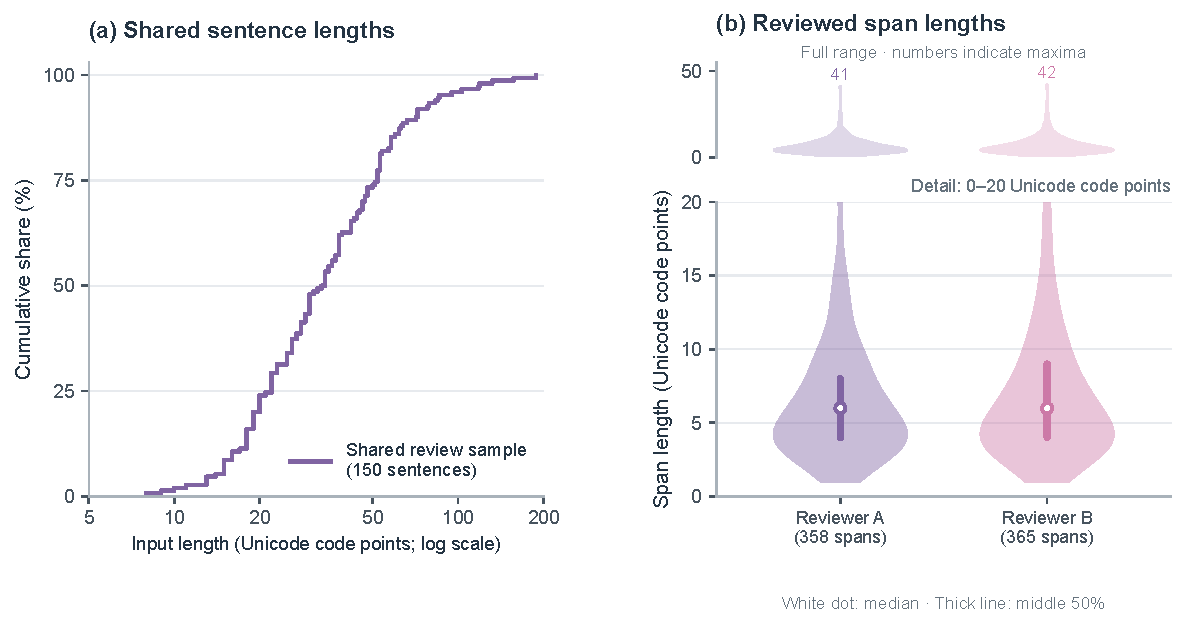
\includegraphics[width=\linewidth]{figures/additional_review_profile_20261006.pdf}
\caption{Length distributions in the additional assisted-review sample. Panel (a) uses the same 150 sentences for both reviewers; panel (b) shows their separate annotation layers, with 358 spans for A and 365 for B. Densities use all observed spans with equal maximum widths. The overview shows the full range of span lengths, while the detail view focuses on 0--20 Unicode code points. Dots mark medians, and thick lines mark the middle 50\%. Supervision and human-reference distributions appear in Figure~\ref{fig:length-distributions-r40}; reviewer-specific type counts appear in Table~\ref{tab:additional-review-composition}.}
\label{fig:additional-review-distributions}
\end{figure}

Table~\ref{tab:additional-review-composition} gives both reviewers' type counts. Table~\ref{tab:qa150-pairs} compares pre-adjudication span sets. Its 95\% percentile intervals use 10,000 sentence resamples within source strata, with source quotas fixed.

\begin{table}[htbp]
\caption{Competency composition in the additional review sample: span counts (within-reviewer percentages).}
\label{tab:additional-review-composition}
\centering\small
\begin{tabular}{@{}lrrrrr@{}}
\toprule
Reviewer & L & S & K & T & Total spans \\
\midrule
A & 3 (0.8\%) & 217 (60.6\%) & 77 (21.5\%) & 61 (17.0\%) & 358 \\
B & 3 (0.8\%) & 218 (59.7\%) & 81 (22.2\%) & 63 (17.3\%) & 365 \\
\bottomrule
\end{tabular}
\end{table}

\begin{table}[htbp]
\caption{Typed exact-span agreement in the additional review sample.}
\label{tab:qa150-pairs}
\centering\small
\begin{tabularx}{\linewidth}{@{}Lccc@{}}
\toprule
Comparison & Exact F1 & 95\% CI & \makecell{Sentences with\\identical span sets} \\
\midrule
Reviewer A--Reviewer B & 0.816 & [0.769, 0.860] & 101/150 \\
Codex--Cursor suggestions & 0.962 & [0.937, 0.983] & 138/150 \\
Reviewer A--Codex suggestions & 0.823 & [0.776, 0.866] & 100/150 \\
Reviewer B--Codex suggestions & 0.850 & [0.803, 0.892] & 108/150 \\
\bottomrule
\end{tabularx}
\par\smallskip\footnotesize\RaggedRight
F1 is micro-averaged; CIs are 95\% percentile intervals from a source-stratified sentence bootstrap.
\end{table}

Agreement uses both reviewers' complete annotation layers, including the 49 sentences with differing span sets. Character-level calculations assign O/L/K/S/T to the original Unicode-code-point positions, including spaces and punctuation. Two positions have conflicting types within one reviewer's layer; excluding them from both character sequences leaves $N=5{,}990$ positions. All original spans remain in span-level F1. The accompanying agreement data identify the affected record. Later adjudication and incorporation into training targets have not been verified. Agreement over the retained character positions is $p_o=0.934$, with $p_e=0.439$ and $\kappa=0.883$.

For nominal Krippendorff's $\alpha$, let $m_c$ count assignments to category $c$ across both reviewers, with $\sum_c m_c=2N$. The observed and expected disagreements are
\begin{equation}
\alpha=1-\frac{D_o}{D_e},\qquad
D_o=1-p_o,\qquad
D_e=1-\frac{\sum_c m_c(m_c-1)}{2N(2N-1)}.
\label{eq:qa150-alpha}
\end{equation}
Here $D_o=0.066$ and $D_e=0.560$, giving $\alpha=0.883$. Character coefficients include the many O positions, whereas span F1 assesses complete spans~\citep{artstein2008agreement}. The machine--machine comparison measures concordance between the suggestion layers.

\subsection{Blinded Coding by Three Annotators}
The annotators were one human resource management specialist with a doctorate and two working professionals pursuing master's degrees in management. The students had sustained annotation experience and three to five years of professional experience. All three contributed to handbook development; two professors advised on the coding process and handbook preparation.

The formal sample comprises eight listed-company, 16 public-institution, and 26 Tianchi sentences from the silver annotation candidates, with one sentence per advertisement identifier. The team reports random selection, although the candidate frame and sampling log are unavailable; the released annotations identify the sampled sentences and sources. Preparation used five familiarization and 15 practice sentences, all excluded from the agreement analysis. The available records do not establish whether all annotators followed the same sequence.

\begin{sloppypar}
The annotators coded independently and could review their own labels using the study handbook, with machine suggestions and other annotators' labels hidden throughout. The main analysis uses each annotator's individual annotations after self-review, as confirmed by the authors, and includes all 50 sentences and all annotator pairs. Mean pairwise typed exact-span F1 is 0.818; the annotations were not adjudicated into a consensus reference. Earlier individual annotations yielded 0.663. Both sets are available in the \href{https://github.com/AlfredJamesLi/chinese-skillspan-benchmark/tree/main/reproduction/style_revision_20261005}{reproduction notes}, but the recorded timing does not establish a comparable before-and-after sequence across annotators. \hyperref[sec:guide-version-history]{Appendix A.4} distinguishes the handbook records from later reader editions. The sample overlaps with expanded-model training data (\hyperref[app:d]{Appendix D}); historical model-reference labels remain unchanged.
\end{sloppypar}

Annotators A, B, and C produced 104, 123, and 113 spans, respectively. Exact typed matches number 90 for A--B, 92 for A--C, and 96 for B--C. O covers 63.2--64.1\% of character positions.

% Detailed blinded-agreement evidence relocated from the corpus chapter.
\phantomsection
\label{sec:blinded-agreement-details}

For typed exact-span F1, a match requires identical boundaries and types, and the two annotators are treated symmetrically~\citep{hripcsak2005agreement}. Boundary-only exact-span F1 ignores type. Character-level agreement uses pairwise Cohen's $\kappa$ and three-annotator nominal Krippendorff's $\alpha$ on L/K/S/T/O assignments to all 2,111 source Unicode code points; O denotes positions outside annotated spans. Character-level coefficients summarize agreement at each position, while span-level F1 requires complete span matches~\citep{artstein2008agreement}.

The 95\% percentile confidence intervals use 10,000 sentence-bootstrap samples drawn within source strata, with all three annotation layers retained together for each sampled sentence. They summarize variation within the sampled strata for these three annotators. Table~\ref{tab:blinded-agreement-pairs} gives the pairwise comparisons underlying Table~\ref{tab:quality-main}.

\begin{table}[!htbp]
\caption{Pairwise agreement on the 50-sentence blinded sample after individual self-review.}
\label{tab:blinded-agreement-pairs}
\centering\small
\setlength{\tabcolsep}{4pt}
\begin{tabularx}{\linewidth}{@{}P{.14\linewidth}P{.26\linewidth}P{.22\linewidth}P{.16\linewidth}L@{}}
\toprule
Pair & Typed exact F1 [95\% CI] & Boundary-only exact F1 & Cohen's $\kappa$ & \makecell[l]{Identical\\span sets\\(sentences)} \\
\midrule
A--B & 0.793 [0.694, 0.884] & 0.828 & 0.880 & 36/50 \\
A--C & 0.848 [0.752, 0.926] & 0.876 & 0.930 & 39/50 \\
B--C & 0.814 [0.721, 0.899] & 0.847 & 0.909 & 37/50 \\
\bottomrule
\end{tabularx}
\par\smallskip
{\footnotesize\RaggedRight F1 compares complete spans; identical span sets include empty sets. Cohen's $\kappa$ uses L/K/S/T/O labels at source character positions. CIs are 95\% percentile confidence intervals.\par}
\end{table}

Mean pairwise typed exact-span F1 was 0.818 (95\% CI [0.732, 0.894]), and boundary-only exact-span F1 was 0.850 (95\% CI [0.766, 0.923]). By type, pairwise F1 ranges were 0.762--0.805 for K, 0.778--0.869 for S, and 0.865--1.000 for T. Character-level $\alpha$ was 0.907 (95\% CI [0.851, 0.954]).

All three annotators produced identical complete typed-span sets for 34 sentences, including 11 with no annotated spans. They also identified the same two L spans, both in one sentence, providing limited evidence about agreement on this category. Individual annotation exports and diagnostics are available in the \href{https://github.com/AlfredJamesLi/chinese-skillspan-benchmark/tree/main/reproduction/agreement/finalguide_abc_20261003}{reproduction materials}.


\subsection{Silver Labels against Blinded Annotations}
We compared the final expanded-pool labels with each of the three blinded annotation layers on the same 49 retained sentences (Table~\ref{tab:silver-blinded}). One of the 50 study sentences remained unresolved at the candidate stage and was absent from both final pools; it was excluded from this comparison rather than scored as an empty annotation. Each per-annotator score pools exact boundary-and-type matches across the 49 sentences, and the mean averages the three micro-F1 scores.

\begin{table}[!htbp]
\centering\small
\caption{Agreement between final expanded Silver labels and individual blinded annotations.}
\label{tab:silver-blinded}
\begin{tabularx}{\linewidth}{@{}Lrrrrr@{}}
\toprule
Silver pool & Sentences & Annotator A & Annotator B & Annotator C & Mean \\
\midrule
Adopted expanded pool & 49 & 0.724 & 0.681 & 0.721 & 0.709 \\
Alternative expanded pool & 49 & 0.723 & 0.716 & 0.721 & 0.720 \\
\bottomrule
\end{tabularx}
\par\smallskip\footnotesize\RaggedRight
Values are typed exact-span micro-F1; the mean is taken across annotators A--C.
\end{table}

This post hoc analysis compares historical silver labels with human annotations made without access to machine suggestions. It complements the assisted reviews, but its findings apply to the selected sample and participating annotators and do not estimate accuracy across the full silver pool. Counts, input hashes, and code are provided in the \href{https://github.com/AlfredJamesLi/chinese-skillspan-benchmark/tree/main/reproduction/reviewer_revision_20261005}{reproduction materials}. The original 150-sentence model scores are unchanged.

\FloatBarrier
